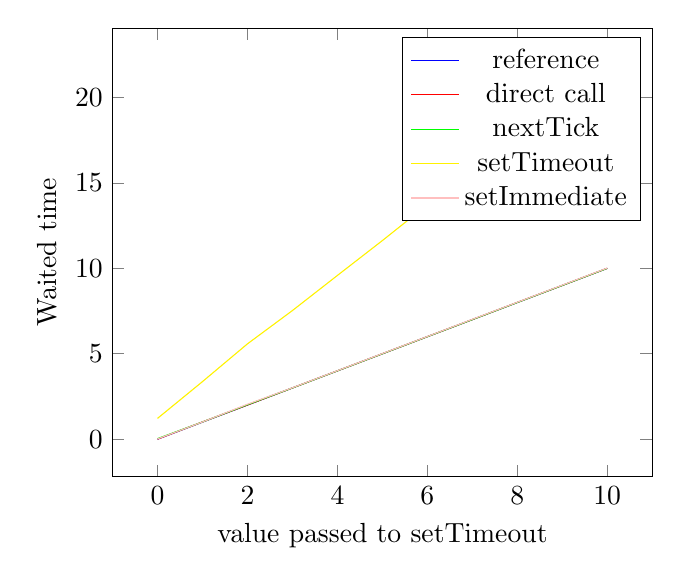
\begin{tikzpicture}
\begin{axis}[xlabel = value passed to setTimeout, ylabel = Waited time]
\addplot[color = blue] coordinates {(0, 0) (1, 1) (2, 2) (3, 3) (4, 4) (5, 5) (6, 6) (7, 7) (8, 8) (9, 9) (10, 10) (0, 0) (1, 1) (2, 2) (3, 3) (4, 4) (5, 5) (6, 6) (7, 7) (8, 8) (9, 9) (10, 10) (0, 0) (1, 1) (2, 2) (3, 3) (4, 4) (5, 5) (6, 6) (7, 7) (8, 8) (9, 9) (10, 10) (0, 0) (1, 1) (2, 2) (3, 3) (4, 4) (5, 5) (6, 6) (7, 7) (8, 8) (9, 9) (10, 10)};
\addplot[color = red] coordinates {(0, 0.002196078431372549) (1, 1.0105882352941176) (2, 2.0009607843137256) (3, 3.0005882352941176) (4, 4.001941176470588) (5, 5.001) (6, 6.0025490196078435) (7, 7.000901960784314) (8, 8.005254901960784) (9, 9.001686274509805) (10, 10.004137254901961)};
\addplot[color = green] coordinates {(0, 0.03309803921568628) (1, 1.0078235294117648) (2, 2.0190980392156863) (3, 3.000921568627451) (4, 4.001450980392157) (5, 5.001607843137255) (6, 6.001607843137255) (7, 7.001921568627451) (8, 8.002607843137255) (9, 9.002156862745098) (10, 10.002588235294118)};
\addplot[color = yellow] coordinates {(0, 1.2185490196078432) (1, 3.372078431372549) (2, 5.581686274509804) (3, 7.530509803921569) (4, 9.585882352941177) (5, 11.626980392156863) (6, 13.721254901960783) (7, 15.884588235294117) (8, 17.812098039215687) (9, 19.902627450980393) (10, 21.86978431372549)};
\addplot[color = pink] coordinates {(0, 0.018294117647058822) (1, 1.0066666666666666) (2, 2.0476666666666667) (3, 3.010470588235294) (4, 4.010509803921568) (5, 5.01313725490196) (6, 6.011333333333333) (7, 7.017921568627451) (8, 8.014803921568628) (9, 9.01707843137255) (10, 10.016882352941176)};
\legend{reference, direct call, nextTick, setTimeout, setImmediate};
\end{axis}
\end{tikzpicture}
